%%%%%%%%%%%%%%%%%%%%%%%%%%%%%%%%%%%%%%%%%
% Beamer Presentation
% LaTeX Template
% Version 1.0 (10/11/12)
%
% This template has been downloaded from:
% http://www.LaTeXTemplates.com
%
% License:
% CC BY-NC-SA 3.0 (http://creativecommons.org/licenses/by-nc-sa/3.0/)
%
%%%%%%%%%%%%%%%%%%%%%%%%%%%%%%%%%%%%%%%%%

%----------------------------------------------------------------------------------------
%	PACKAGES AND THEMES
%----------------------------------------------------------------------------------------

\documentclass{beamer}

\mode<presentation> {

% The Beamer class comes with a number of default slide themes
% which change the colors and layouts of slides. Below this is a list
% of all the themes, uncomment each in turn to see what they look like.

%\usetheme{default}
%\usetheme{AnnArbor}
%\usetheme{Antibes}
%\usetheme{Bergen}
%\usetheme{Berkeley}
%\usetheme{Berlin}
%\usetheme{Boadilla}
%\usetheme{CambridgeUS}
%\usetheme{Copenhagen}
%\usetheme{Darmstadt}
%\usetheme{Dresden}
%\usetheme{Frankfurt}
%\usetheme{Goettingen}
%\usetheme{Hannover}
%\usetheme{Ilmenau}
%\usetheme{JuanLesPins}
%\usetheme{Luebeck}
%\usetheme{Madrid}
%\usetheme{Malmoe}
%\usetheme{Marburg}
%\usetheme{Montpellier}
%\usetheme{PaloAlto}
\usetheme{Pittsburgh}
%\usetheme{Rochester}
%\usetheme{Singapore}
%\usetheme{Szeged}
%\usetheme{Warsaw}

% As well as themes, the Beamer class has a number of color themes
% for any slide theme. Uncomment each of these in turn to see how it
% changes the colors of your current slide theme.

%\usecolortheme{albatross}
%\usecolortheme{beaver}
%\usecolortheme{beetle}
%\usecolortheme{crane}
%\usecolortheme{dolphin}
%\usecolortheme{dove}
%\usecolortheme{fly}
%\usecolortheme{lily}
%\usecolortheme{orchid}
%\usecolortheme{rose}
%\usecolortheme{seagull}
%\usecolortheme{seahorse}
%\usecolortheme{whale}
%\usecolortheme{wolverine}

%\setbeamertemplate{footline} % To remove the footer line in all slides uncomment this line
%\setbeamertemplate{footline}[page number] % To replace the footer line in all slides with a simple slide count uncomment this line

%\setbeamertemplate{navigation symbols}{} % To remove the navigation symbols from the bottom of all slides uncomment this line
}

\usepackage{graphicx} % Allows including images
\usepackage{booktabs} % Allows the use of \toprule, \midrule and \bottomrule in 
\usepackage{amsfonts,amsmath,amssymb,graphicx,url}
\usepackage{comment}
%----------------------------------------------------------------------------------------
%	TITLE PAGE
%----------------------------------------------------------------------------------------

\title[Short title]{Project On Parameterization} % The short title appears at the bottom of every slide, the full title is only on the title page

\author{Xuan Li} % Your name
\institute[CS@SBU] % Your institution as it will appear on the bottom of every slide, may be shorthand to save space
{
Stony Brook University \\ % Your institution for the title page
\medskip
\textit{xuanli2@cs.stonybrook.edu} % Your email address
}
\date{\today} % Date, can be changed to a custom date

\begin{document}

\begin{frame}
\titlepage % Print the title page as the first slide
\end{frame}
\begin{frame}
\footnotesize{
\begin{thebibliography}{99} % Beamer does not support BibTeX so references must be inserted manually as below
\bibitem[Aigerman, 2015]{p1} Noam Aigerman, Yaron Lipman  (2015)
\newblock Orbifold Tutte Embeddings
\newblock \emph{ACM Transactions on Graphics (TOG) - Proceedings of ACM SIGGRAPH Asia 2015, 34(6)}
\bibitem[Aigerman, 2016]{p1}
Noam Aigerman, Yaron Lipman (2016)
\newblock Hyperbolic Orbifold Tutte Embeddings
\newblock \emph{ACM Transactions on Graphics (TOG) - Proceedings of ACM SIGGRAPH Asia 2016, 35(6)}
\bibitem[Sawhney, 2017]{p1}
Rohan Sawhney, Keenan Crane (2017)
\newblock Boundary First Flattening
\newblock \emph{ACM Transactions on Graphics (TOG) (Under Review)}
\end{thebibliography}
}
\end{frame}

\begin{frame}
\frametitle{Overview} % Table of contents slide, comment this block out to remove it
\tableofcontents % Throughout your presentation, if you choose to use \section{} and \subsection{} commands, these will automatically be printed on this slide as an overview of your presentation
\end{frame}

%----------------------------------------------------------------------------------------
%	PRESENTATION SLIDES
%----------------------------------------------------------------------------------------

%------------------------------------------------
\section{Project Overview} % Sections can be created in order to organize your presentation into discrete blocks, all sections and subsections are automatically printed in the table of contents as an overview of the talk
%------------------------------------------------
\begin{frame}
\frametitle{Project Conponents}
\textbf{Orbifold Embedding} 

Generalization of Tutte embedding to sphere-type mesh. 

I explore two kinds of background geometry: Euclidean and hyperbolic.
~\\
~\\
\textbf{Boundary First Flattening}

Based on differential geometry.

Conformal map. 

Handle curvature and conformal factors directly.

With cone technique, can be generalize to meshes with slices.
  
\end{frame}


\section{Orbifold Tutte Embeddding} % A subsection can be created just before a set of slides with a common theme to further break down your presentation into chunks


\begin{frame}
\frametitle{Tutte Embedding}
The embedding problem is the following full-rank linear system:
\begin{equation}
\begin{split}
\sum_{v_j \in \mathit{N}(v_i)} w_{ij}(z_j-z_i) &= 0, \ \  v_i \in V - B\\
z_i &= z_i^0, \ \ v_i \in B\\
\end{split}
\label{eq:tutte}
\nonumber
\end{equation}
where $w > 0$.

\textbf{Harmonic Map:} $w_{ij} = \frac{\cot \alpha_{ij} + \cot \beta_{ij}}{2}$ 

\begin{figure}
\centering
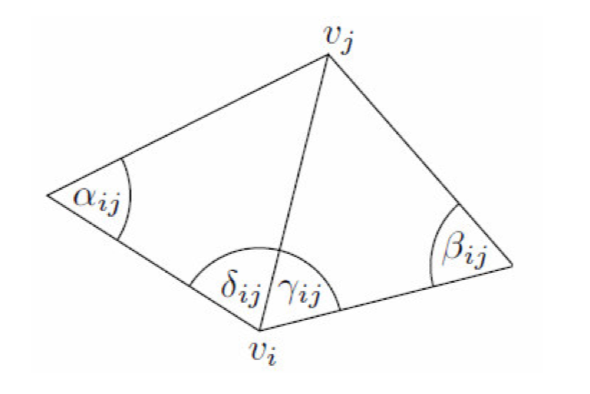
\includegraphics[width = 0.3\textwidth]{images/harmonic}
\end{figure}

\end{frame}


\begin{frame}
\frametitle{Tutte Embedding Equivalence}
\begin{equation}
\begin{split}
&\min_{\Phi}\ \ \   E(z) = \frac{1}{2}\sum_{(i,j)\in E} w_{ij} d(z_i, z_j)^2 \\
s.t \ \ \   &z_i = z_i^0, \ \ \ \ v_i \in B
\end{split}
\nonumber
\end{equation}
\end{frame}

\begin{frame}
\frametitle{Orbifold}
Tiled space defined by a basic tile.

Points differed by a transition between copies are equivlence.

Transition: rigid motions.

\begin{figure}
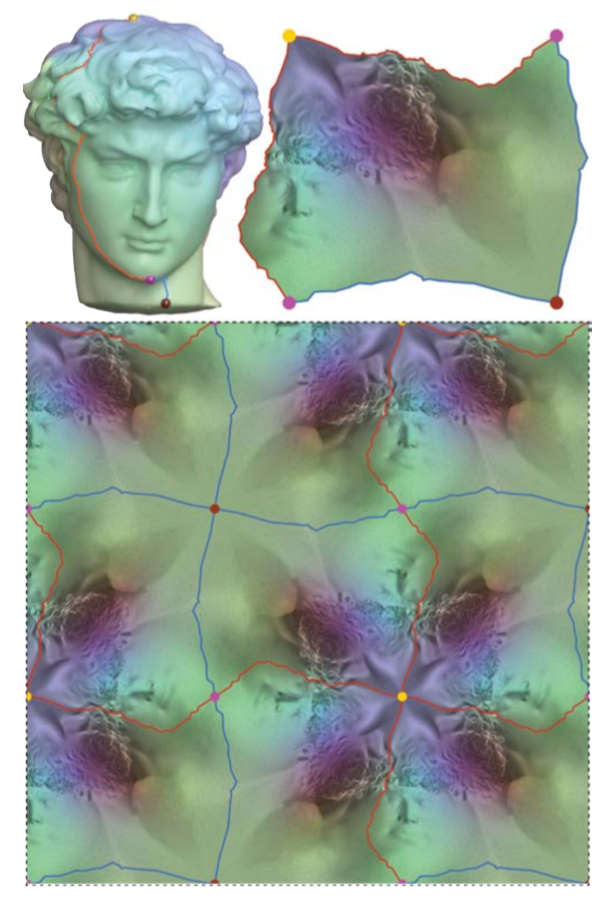
\includegraphics[width=0.3\textwidth]{images/euclidean-orbifold.png}
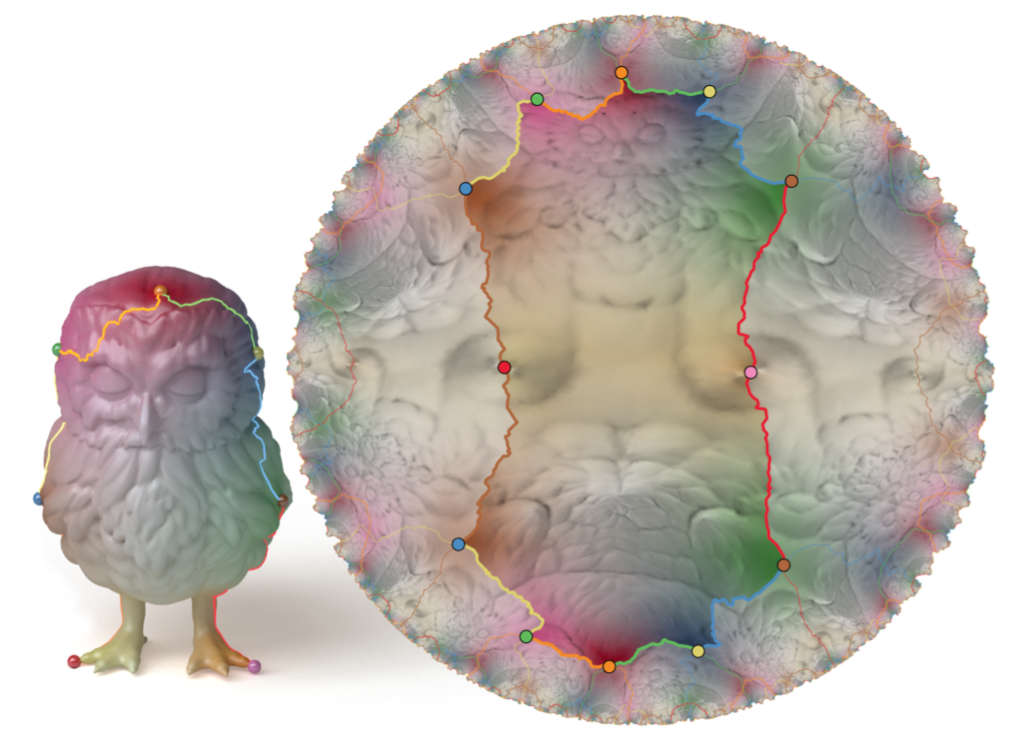
\includegraphics[width=0.5\textwidth]{images/hyperbolic-orbifold.png}
\end{figure}
\end{frame}

\begin{frame}
\frametitle{Euclidean Orbifold Tutte Embedding}
Select some cones and cut the mesh into a disk, we solve:

For $v_i \in \bar{V}-\bar{B}$: $$ \sum_{v_j \in N(v_i)}w_{ij}(z_j - z_i) = 0 $$
For $(v_i, v_{i'})\ \text{boundary pair}$,
$$\begin{matrix}
\sum_{v_j \in N(v_i)}w_{ij}(z_j - z_i) + \sum_{v_j\in N(v_{i'})} w_{i'j}R_{i'i}(z_j - z_{i'})  = 0\\
R_{i'i}z_{i'} - z_i  = t_{ii'} 
\end{matrix} $$
For $v_i \in \bar{C}$,
$$z_i = z_i^0  $$
\end{frame}

\begin{frame}
\frametitle{Hyperbolic Tutte Embedding}
\begin{equation}
\begin{split}
&\min_{\Phi} E(z),\\
s.t \ \ \ &z_i = m_{i'i}(z_{i'}), \ \ \ \ v_i \in \bar{B} - \bar{C}\\
 &z_i = z_i^0, \ \ \ \ v_i \in \bar{C}\\
\end{split}
\nonumber
\end{equation}

The gradient of the energy is given by
\begin{equation}
\nabla_{z_i} E = \sum{j\in N_i}  w_{ij}\nabla_{z_i}d^2(z_i, z_j) + \sum{j\in N_{i'}}w_{i'j}\nabla_{z_i}d^2(z_i, m_{i'i}(z_j))
\nonumber
\end{equation}

\end{frame}



\section{Boundary First Flattening}
\begin{frame}
\frametitle{Poisson Problems}
Dirichlet-type condition:
\begin{equation}
\begin{split}
\Delta a &= \phi \ \ \ \ \ \  on\  M\\
a &= g , \ \ \  on\ \partial M
\end{split}
\end{equation}
Riemann-type condition:
\begin{equation}
\begin{split}
\Delta a &= \phi \ \ \ \ \ \  on\  M\\
\frac{\partial a}{\partial n} &= h , \ \ \  on\ \partial M 
\end{split}
\end{equation}

Discrete version (Riemann):
\begin{equation}
\left[\begin{matrix}
A_{II} & A_{IB}\\
A_{BI} & A_{BB}
\end{matrix}\right] \left[\begin{matrix}
a_I\\
a_B
\end{matrix}\right]
= \left[\begin{matrix}
\phi_I\\
\phi_B - h\end{matrix}\right]
\label{eq:relation}
\end{equation}

\end{frame}

\begin{frame}
\frametitle{Conversion between Dirichlet and Riemann}
Given $h$, we simply solve the Poisson equation and set 
\begin{equation}
g = \Lambda^*_\phi h = a_B,
\end{equation}
Given $g$, we can convert it to $h$  by
\begin{equation}
h = \Lambda_\phi g = \phi_B - A_{IB}^TA_{II}^{-1}(\phi_I - A_{IB}g) - A_{BB}g
\end{equation}
\end{frame}

\begin{frame}
\frametitle{Cherrier Formula}
For a conformal map $f: M \rightarrow \tilde{M}$, we have 
\begin{equation}
\begin{split}
\Delta u = K - e^{2u} \tilde{K} \ \ \ &on\ M\,\\
\frac{\partial u}{\partial n} = k - e^{u}\tilde{k} \ \ \ &on\     \partial M
\end{split}
\end{equation}
where $u$ is conformal factor, $K$,$\tilde{K}$ are Gauss curvature of the source surface and  the target surface, $k, \tilde{k}$ is geodesic curvature of the source surface and the target surface.


\end{frame}

\begin{frame}
\frametitle{Discrete Cherrier Formula}
\begin{equation}
\begin{split}
Au &=   \Omega - \tilde\Omega\  \ \ on\  Int\  M\\
h &= k - \tilde{k} \ \ \  on\ \partial M 
\end{split}
\label{eq:poisson}
\end{equation}
where $\Omega_i = 2\pi - \sum_{ijk \in F}\theta_i^{jk}$ defined on interior vertices, $k_i = \pi - \sum_{ijk \in F}\theta_i^{jk}$ defined on boundary vertices, which is the exterior angle at $v_i$. Note that $\Omega$ is defined to be zero at boundary vertices.
\end{frame}

\begin{frame}
\frametitle{Algorithm}
The pipeline of the BFF algorithm is as follows:

1) If boundray conformal factor ${u}$ is known, we compute bounadry target $k$ by: $$ \tilde{k} = k -\Lambda_{\Omega} u.$$
If target boundary $\tilde{k}$ is known, we compute boundary conformal factor $u$ by:: $$u = \Lambda_{\Omega}^{*}(k - \tilde{k}).$$

2) Define new boundary edge lengths as:
$$l_{ij}^* = e^{\frac{u_i + u_j}{2}}l_{ij}.$$ With $\tilde{k}$, which is exterior angles, we can integrate these two data into a closed loop.

3) Extend the loop into interior conformally.
\end{frame}

\begin{frame}
\frametitle{Loop Integration}
In step 2, usually, directly integrating $\tilde{k}$ over $l_{ij}^*$ won't give a closed loop, we should change edge length a little. So we solve the following quadratic optimization problem:

\begin{equation}
\begin{split}
&\min_{\tilde{l}}\ \  ||\tilde{l} - l^*||^2_2\\
s.t. & \sum_{ij\in \partial M} \tilde{l}_ij \tilde{T}_{ij}
\end{split}
\end{equation}
\end{frame}



\begin{frame}
\frametitle{Conformal Interpolation}
Two choice:

1) Use harmonic map on both components

2) Use harmonic map on one componet, and minimize conformal energy on the other component. Linear problem.
\end{frame}

\begin{frame}
\frametitle{Video Demo}
GitHub: xuan-li (\url{https://github.com/xuan-li/GraphicsProject})

\end{frame}

%----------------------------------------------------------------------------------------

\end{document}